% Preamble
\documentclass[../Relazione_circuiti]{subfiles}

% Packages

\graphicspath{{\subfix{../images/}}}

% Document
\begin{document}

\begin{minipage}{.49\textwidth}
  \setlength{\parindent}{20pt}
  Per effettuare l'esperimento abbiamo utilizzato:
  \begin{itemize}
    \item Scheda Elvis II della National Instruments
    \item Computer
    % le ~ servono a non far andare a capo tra valore e unità di misura
    \item Due resistenze ($99.76 \pm 0.05$~\textOmega \hspace{1pt} su ramo Tweeter e $99.59 \pm 0.05$~\textOmega
    \hspace{1pt} su ramo Woofer), un condensatore ($1.03 \pm 0.01 $~\textmu F) e un'induttanza ($11.8 \pm 0.1$~mH)
  \end{itemize}

  La scheda millefori della Elvis ha fatto da base per il circuito, che è poi stato alimentato dal suo function
  generator, e tutte le misure sono state effettuate tramite il multimetro digitale e l'analog input multicanale sempre
  della Elvis (si veda l'appendice\,\ref{sec:errori_strumentali} per il calcolo delle incertezze su questi dati).

  Il computer si è interfacciato con la scheda per gestire le operazioni di misura.
\end{minipage}
\hfill
\begin{minipage}{0.50\textwidth}
  \centering
  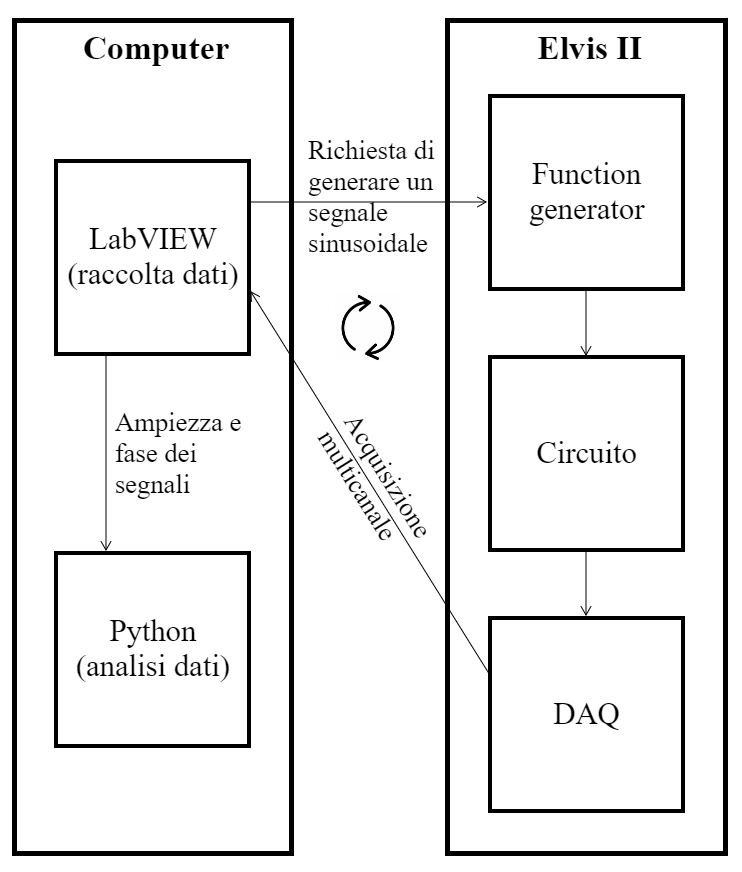
\includegraphics[width=.93\textwidth]{Pipeline_scheme.png}
  \captionof{figure}{\label{fig:schema_pipeline}Schema acquisizione bufferizzata}
\end{minipage}\vspace{1mm}
\indent La componentistica elettrica è stata usata per realizzare il circuito.

È importante notare la bassa resistenza dell'induttanza utilizzata, trascurabile rispetto alle resistenze di carico
(circa $1$ \textOmega), necessaria per la validità di tutte le formule utilizzate in questo articolo.

\subsection{Misure effettuate}\label{subsec:misure-effettuate}

  Per misurare la resistenza interna del function generator della Elvis abbiamo messo una resistenza nota $R$ ai capi
  del generatore e misurato 299 volte la caduta di potenza su di essa, prendendo poi la media $V$, e calcolato
  \begin{equation*}
    Rg = R \left( \frac{ddp}{V} - 1 \right)
  \end{equation*}
  dove $ddp$ è la differenza di potenziale richiesta al generatore. \\ \\
  \begin{minipage}{0.49\textwidth}
    \setlength{\parindent}{20pt}
    Abbiamo poi impostato l'acquisizione dati come in Tab\,\ref{tab:parametri-daq} e con questi parametri abbiamo
    misurato:
    \begin{itemize}
      \item La differenza di potenziale tra il generatore e il ground
      \item La caduta di potenziale sulle resistenze di carico
    \end{itemize}

  \end{minipage} \hfill
  \begin{minipage}{0.49\textwidth}

    \centering
    \begin{minipage}{0.85\textwidth}
      \centering
      \begin{tabular}{|c|c|}
        % Par name & Par val
        \hline
        Sample per buffer & 3000                           \\
        Sample al secondo & $ 450 \cdot 10^3 $             \\
        Range             & 200 Hz − 10 kHz                \\
        Passo             & $\nu_{i+1} = \nu_i \cdot 1.01$ \\ \hline
      \end{tabular}

      \captionof{table}{Parametri per acquisizioni bufferizate}
      \label{tab:parametri-daq}
    \end{minipage}

  \end{minipage} \\
  
  Il range di acquisizione consente di ottenere curve simmetriche rispetto alla frequenza di cross per ampiezza e fase. L'incremento moltiplicativo è tale da generare un incremento  di step costante in scala logaritmica. La sample rate consente di acquisire con precisione le forme d'onda in tutto il range di scansione.

  Da questi dati abbiamo estratto con un fit della forma $ A \sin\left( \omega t + \phi \right) $ i valori di ampiezza e
  fase (come frequenza abbiamo usato quella del function generator, nota con un'incertezza assoluta di 0.186 Hz), che
  abbiamo utilizzato nella fase di analisi (Si veda la Fig.\,\ref{fig:schema_pipeline} per uno schema del processo
  descritto)

\end{document}